\documentclass[10pt]{report}


\usepackage{latexsym}
\usepackage{amsmath}
\usepackage{amssymb}
\usepackage{amsfonts}
\usepackage{amsthm}
\usepackage{amscd}
\usepackage{epsfig}
\usepackage{verbatim}
\usepackage{fancybox}
\usepackage{moreverb}
\usepackage{graphicx}
\usepackage{psfrag}
\usepackage{hyperref}
\usepackage[all]{xy}
\usepackage[toc,page]{appendix}
\usepackage[subnum]{cases}
\usepackage{bm}
\usepackage{framed}
\usepackage{color}
\usepackage{dsfont}
\usepackage{textcomp}
\usepackage{graphicx}
\usepackage{url}
\usepackage[francais]{babel}
\usepackage[utf8]{inputenc}  
\usepackage[T1]{fontenc}
\usepackage[top=2cm, bottom=2cm, left=2cm, right=2cm]{geometry}
\usepackage{epstopdf}
\usepackage{epsfig}
\usepackage{listings}

%\textheight 22cm    \textwidth 16cm
%\voffset = 0 cm
%\hoffset = 0 cm
%\marginparwidth = 0pt
%\oddsidemargin = 31pt
%one inch + \hoffset
%one inch + \voffset
%\oddsidemargin = 31pt
%\topmargin = 20pt
%\headheight = 12pt
%\headsep = 25pt
%\textheight = 592pt
%\textwidth = 390pt
%\marginparsep = 10pt
%\marginparwidth = 35pt
%\footskip = 30pt
%\marginparpush = 7pt
%\hoffset = 0pt
%\voffset = 0pt
%\paperwidth = 597pt
%\paperheight = 845pt


\newcommand{\C}{{\mathbb C}}
\newcommand{\R}{{\mathbb R}}
\newcommand{\N}{{\mathbb N}}
\newcommand{\Z}{{\mathbb Z}}
\newcommand{\Q}{{\mathbb Q}}
\newcommand{\T}{{\mathbb T}}
\newcommand{\E}{{\mathbb E}}
\newcommand{\di}{{\mathbb D}}
\newcommand{\Y}{{\mathbf Y}}
\newcommand{\D}{{\partial}}
\newcommand{\Cl}{{\mathcal C}}
\newcommand{\Pa}{{\mathcal P}}
\newcommand{\Flux}{{\mathcal F}}
\newcommand{\B}{{\mathfrak B}}
\newcommand{\M}{{\mathcal M}}
\newcommand{\dis}{{\mathcal D}}
\newcommand{\A}{{\mathcal{A}}}
\newcommand{\fin}{\rule{1ex}{1ex}}
\newcommand{\HRule}{\rule{\linewidth}{0.5mm}}
\renewcommand\labelitemi{\textbullet}

\newtheorem{theorem}{Theorem}
\newtheorem*{theorem*}{Theorem}
\newtheorem{lemma}[theorem]{Lemma}
\newtheorem*{lemma*}{Lemma}
\newtheorem{proposition}[theorem]{Proposition}
\newtheorem*{proposition*}{Proposition}
\newtheorem{corollary}[theorem]{Corollary}
\newtheorem{definition}[theorem]{Definition}
\newtheorem*{definition*}{Definition}
\newtheorem{example}[theorem]{Example}
\newtheorem{remark}[theorem]{Remark}
\newtheorem{notation}[theorem]{Notation}
\newtheorem{hypothesis}[theorem]{Hypothesis}


\renewcommand{\thesection}{\arabic{section}}
\renewcommand{\thelemma}{\thesection\arabic{lemma}}
\renewcommand{\theproposition}{\thesection\arabic{proposition}}
\renewcommand{\thetheorem}{\thesection\arabic{theorem}}
\renewcommand{\thecorollary}{\thesection\arabic{corollary}}
\renewcommand{\thedefinition}{\thesection\arabic{definition}}
\renewcommand{\theexample}{\thesection\arabic{example}}
\renewcommand{\theremark}{\thesection\arabic{remark}}
\renewcommand{\thenotation}{\thesection\arabic{notation}}
\renewcommand{\theequation}{\thesection.\arabic{equation}}
\def\commutatif{\ar@{}[rd]|{\circlearrowleft}}


\begin{document}

\begin{titlepage}

\begin{center}


% Upper part of the page

\includegraphics[scale = 0.7]{Logolille1.jpg}
\hspace{6.4cm}

\includegraphics[scale = 0.4]{LogoUWO.png}
\\[1cm]    


\href{http://mathematiques.univ-lille1.fr/Formation/Masters-de-l-UFR-de-Mathematiques/Masters-ingenierie-mathematiques/Master-2-specialite-scientific-computing/}{\large \textcolor{blue}{Master degree in Mathematical Engineering (Advanced Scientific
Computing) of Lille 1}}\\[0.7cm]
\textsc{\LARGE Universities of Lille 1 and Western Ontario}\\[1cm]

\textsc{\Large internship report :}\\[0.3cm]


% Title
\HRule \\[0.4cm]
{ \huge \bfseries Real root isolation for univariate polynomials on GPUs and multicores}\\[0.4cm]

\HRule \\[1cm]

\includegraphics[scale=0.08]{MiddleSexCollege.jpg}\\[1.5cm]

% Author and supervisor
\begin{minipage}{0.4\textwidth}
\begin{flushleft} \large
\emph{Author:}\\
Alexandre \textsc{Temperville}
\end{flushleft}
\end{minipage}
\begin{minipage}{0.4\textwidth}
\begin{flushright} \large
\emph{Supervisor:} \\
Dr. Marc \textsc{Moreno Maza}
\end{flushright}
\end{minipage}

\vfill

% Bottom of the page
\textsc{{\large April 16th - August 16th 2012}}\\
\textsc{{\large Presentation June 16th 2012}}\\


\end{center}

\end{titlepage}

\newpage
\section*{Acknowledgements}
First of all, I thank Marc Moreno Maza to supervise me all these months and also for his welcome, his help, his explanations and all the comments he gave me to improve my work and this paper. I want to thank also all the team of the lab, Chango Chen, Rong Xiao, Anis Sardar Haque and Paul Vrdim for their advices concerning anything, whether it was for the work or for the city, their help and their welcome.\\


I also thank all the professors of the Master Degree of Computer Sciences at Lille 1 for their patience with my questions, their interesting courses, and in particular Chistophe Besse and Nouredine Melab who are the professors in charge of this Master at Lille 1 for letting me discover all this year High Performance Computing and for their involving in this Master allowing me to be put forth my best efforts. I thank also François Lemaire and Adrien Poteaux who coordinates relations between Lille 1 and UWO and for lending one's support to me.\\

I thank also my roomates, Matthew and Raj, who give me a nice stay and also for their kindness, their humour and their friendship. Life in Canada without them would not be the same.\\

To finish I want to thank my family and my friends sending me emails, giving me shouts and news, in particular my little brother Jérôme to help me in english. It was really encouraging from the part of everyone, so thank you everybody.


\renewcommand{\contentsname}{Contents}
\renewcommand{\bibname}{References}
\tableofcontents
% \maketitle




\section*{Introduction}
\newpage

\section{Internship context}
\subsection{University of Western Ontario of London (UWO)}

The University of Western Ontario, located in the city of London and generally called UWO, is among the top 10 Canadian universities.
Renowned for the quality of its students' life,
this university is also worldly ranked between 150 and 300,
from various sources.

\subsection{Departments of Computer Science and Applied Mathematics}
These departments are located in the building called Middlesex College we can see in the presentation page.

\subsection{My supervisor, professor Marc Moreno Maza}

Marc Moreno Maza is an associate professor in the department of Computer Sciences and in the department of Applied Mathematics at the University of Western Ontario. He is also a Principal Scientist in the Ontario Research Centre for Computer Algebra (ORCCA).

Marc Moreno Maza's research activities have four directions :
\begin{itemize}
\item[\textbullet] Study theoretical aspects of systems of polynomial equations and try to answer the question ``what is the best form for the set of solutions?''
\item[\textbullet] Study algorithmic answers to the question ``how to compute this form of the set of solutions at the lowest cost?''
\item[\textbullet] Study implementation techniques for algorithms to make the best use of today's computers.
\item[\textbullet] Apply it to unsolved problems when the prototype solver is ready.
\end{itemize}

\subsection{Maple}

Conforming to the research activities of my supervisor and of the departments of Computer Science and Applied Mathematics, we work in close cooperation with the software company {\it Maplesoft}, which is developing and distributing the computer algebra system {\sc Maple}. Our main purpose is to provide {\sc Maple}'s end-users with symbolic computation tools 
that make best use of computer resources and take advantage of hardware acceleration technologies, in particular graphics processing units (GPUs) and multicores. Marc Moreno Maza's team is currently working on a library called \textit{cumodp} which will be integrated into {\sc Maple} so as to do fast arithmetic operations over prime fields (that is, modulo a prime number).

\subsection{Purpose of my internship}

I participate to the elaboration of the library \textit{cumodp}. My objective is to develop code for the exact calculation of the real roots of  univariate polynomials. Stating this problem is very easy. However, as one dives into the details, one realizes that there are lots of challenges in order to reach highly efficient algorithmic and software solutions.

The first challenge is that of representation. Traditionally, scientific software provide numerical approximations to the roots (real or complex) 
of a univariate polynomial which coefficients might themselves 
be known inaccurately. Nevertheless, in many applications 
polynomial systems 
result from a mathematical model and their coefficients are known exactly.  In this case, it is desirable to obtain closed form formulas for the roots of such polynomials, like $x = \cfrac{1 +/- \sqrt{5}}{2}$
It is well know, however, from Galois Theory, that the roots of
univariate polynomials of degree higher than $4$ cannot
be expressed by radicals.
In this context,
computing the real roots of such a polynomial $f(x) \in {\R}[x]$ means
determining pairwise disjoint intervals with rational end points
and an effective one-to-one map between those intervals and 
the  real roots of $f(x)$.

Algorithms realizing this task are highly demanding in computer
resources. In addition, the most efficient such algorithms
combine different mathematical tools such as Descartes rule
of signs,  Fast Fourier Transforms (FFTs),
continued fractions, computing by homomorphic images, etc.
Therefore, one of my first tasks  when I arrived in London, 
was to learn these techniques which are at the core
of the problem which is proposed to me.



\newpage
\section{Key points of the research of real roots of a univariate polynomial}
\newtheorem*{drs}{Descartes' rule of signs (DRS)}
\newtheorem*{gp}{Gauss' property}
\newtheorem*{tiv}{Theorem of the intermediate values (TIV)}

\subsection{Descartes' rule of signs}

In his 1637 treaty called "La Géométrie", 
René Descartes expressed a rule allowing to estimate 
the number $c$ of positive real roots of a univariate 
polynomial, which we commonly call the Descartes's rule of signs. 
Later, in 1828, Carl Friedrich Gauss proved that if we count 
the roots with their multiplicities, then the number of positive roots 
has the same parity as $c$. 
Usually, Descartes' rule of signs  refers also to the enhancement of Gauss.

\begin{drs}
Let us consider a univariate polynomial $P\in\mathbb{R}[X]$ and the sequence 
$(a_n)$ of its non-zero coefficients. Let $c$ be the number of sign changes 
of the sequence $(a_n)$. Then the number of positive roots of $P$ is at most $c$.
\end{drs}


\begin{gp}
If we consider the previous rule of signs and 
count the roots with their multiplicities, 
then the number of positive real roots of $P$ 
has the same parity than $c$.
\end{gp}

\noindent \textit{Consequence:} We can also find the number of 
negative real roots applying Descartes' rule of signs to $Q(X) = P(-X)$.


This easy rule is the pillar of the reasoning in our work. 
Indeed, deciding where the real roots of a polynomial are located
reduces to the problem  of counting the number of real roots
of a polynomial in an interval.
The example of Section 2.3 illustrates this process.
The following basic theorem plays an essential role in the proof
of Descartes' rule of signs.


\begin{tiv}
If $f$ is a real-valued continuous function on the interval $[a, b]$ and $u$ is a number between $f(a)$ and $f(b)$, then there exists $c\in [a, b]$ such tha we have $f(c) = u$.
\end{tiv}


In particular if $u = 0$, then there  exists $c\in [a, b]$ such that $f(c) = 0$ holds.


\subsection{Horner's method}

This well-known high school tricks is used for evaluating a polynomial
efficiently.
Instead of considering $P(X) = \sum_{i=0}^{n} a_i\, X^i = a_0 + a_1\, X + a_2\, X^2 + ... + a_n\, X^n$, we write $P$ as
$$P(X) = a_0 + X\, \left(a_1 + x\, \left(a_2 + X\,\left(\cdots \left(a_{n-1} + \left(a_n\, X\right)\cdots \right)\right)\right)\right).$$
This allows one to reduce the number of coefficient operation
necessary to evaluate $P(X)$ at a point 
from ${\Theta}(n^2)$ to  ${\Theta}(n)$.
 


\textit{\textbf{Example :}}
Let us consider $P(X) = 3\, X^3 - 5\,X^2 - 3\,X + 2$. We want to calculate $P(4)$ by hand.\\
\underline{Naive method :} $P(4) = 3\times 4^3 - 5\times 4^2 - 3\times 4 + 2$\\
So $P(4) = 3\times 4^3 - 5\times 16 - 12 + 2 = 3\times 16\times 4 - 80 - 10 = 3\times 64 - 90 = 192 - 90 = 102$\\
\underline{Horner's method :} $P(X) = 2 + X\, \left(-3 + X\, \left(-5 + 3\,X \right) \right)$\\
So :
$ P(4) = 2 + 4\, \left(-3 + 4\, \left(-5 + 3\,4 \right) \right) = 2 + 4\, \left(-3 + 4\times 7 \right) = 2 + 4\times 25 = 102 $\\


\subsection{Examples of real root search}
Let us consider $P(X) = X^3 + 3\, X^2 - X - 2$.
According to the Descartes' rule of signs, $c = 1$ so $P$ has $1$ positive root.

Let us consider $Q(X) = P(-X) = -X^3 + 3\, X^2 + X - 2$, here $c = 2$ so $P$ 
has either $2$ or $0$ negative roots. 
We have $P(-1) = 1$ and $\lim_{X \to -\infty} P(X) = -\infty$ 
so there exists $r_{1}\in ]-\infty; -1[$ such that we have $P(r_1) = 0$.


\subsection{Vincent Collins Akritas Algorithm}
To isolate the real roots of a polynomial $P$, our objective is to use the Vincent-Collins-Akritas (VCA) Algorithm which computes a list of disjoint intervals with rational endpoints such that each real root of $P$ belongs to a single interval and each interval contains only one real root of $P$. As mentioned above, the problem of isolating the real roots of $P$ and that of counting its real roots are essentially the same. Therefore, if an algorithm solves one of these two problems, then is solves the other. The following Algorithm 1  (taken from~\cite{CacheComp} uses Algorithm 2 and shows how we can reduce the search  for the roots in $\mathbb{R}$ to the search of the roots in $\left]0, 1\right[$.

\begin{center}
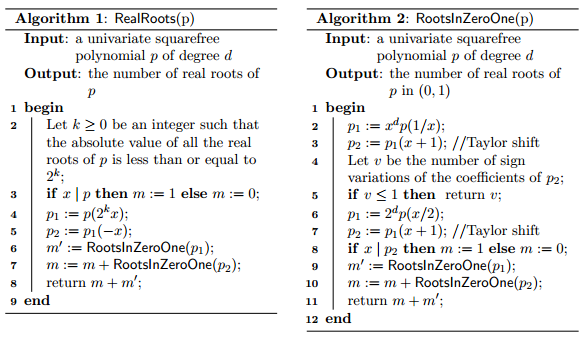
\includegraphics[scale=1]{VCAalgo.png}
\end{center}

Algorithm 1 calls several times the procedure RootsInZeroOne 
which, itself,  performs several times a Taylor shift by 1
(usually called Taylor shift). 
The Taylor shift by $a\in\mathbb{R}$ of a polynomial $P$ 
consists of computing the coefficients of the
polynomial $P(x+a)$ in the monomial basis.
 We will see later what there are differents ways to do this Taylor shift by 1.
Even if evaluating $P(x+1)$ seems an operation mathematically trivial,
non-triavial algorithms have been developed to perform
this operation efficiently on polynomials of large degrees.

Since the dominant computational costs of the VCA Algorithm
comes from the Taylor shift by 1, it is natural
to optimize this operation, in particlar, in terms
of parallelism and data locality.
Of ourse Algorithms 1 and 2, with their divide and conquer 
scheme, seem to provide additional opportunities
for concurrent execution.
However, the work load in the recusrive calls of Algorithms 1 and 2
is generally largely unbalanced, thus, leading to very little
parallelism in practice.

\newtheorem*{crt1}{Chinese Remainder theorem $1^{st}$ version (CRT1)}
\newtheorem*{crt2}{Chinese Remainder theorem $2^{nd}$ version (CRT2)}

\subsection{Modular arithmetic}

Computing with polynomials or matrices over $\mathbb{Z}$ (and thus  $\mathbb{Q}$,
$\mathbb{R}$, $\mathbb{C}$) one generally observes expression swell in the
coefficients.
This phenomenom can be a severe performance bottleneck for computer algebra
software. 
There are essentially two ways to deal with that.
One solution is to use highly optimized multi-precision libraries, such as GMP, 
for computing in  $\mathbb{Z}$ and $\mathbb{Q}$.
Another approach consists in computing by homomorphic images.
One popular way to do this is via (one of the variants of) 
the {\em Chinese Remainder Algorithm}, the other one is to
Hensel's Lemma.
In our work, we rely on the former, see Section 2.6.

Therefore, we replace computations (for instance Taylor shift by 1) 
over $\mathbb{Z}$ by computations over prime fields
of the form $\mathbb{Z}/p{\mathbb{Z}}$ where $p$ has machine word size.
Then it becomes essential to perform efficiently 
arithmetic operations in  $\mathbb{Z}/p{\mathbb{Z}}$.\\

In the C code below, used in my implementation, \textit{sfixn} represents an integer according to the architecture and operating system of the target computer. 
For Linux on Intel 64-bit, \textit{sfixn} is an \textit{int}) and $BASE\_1 = 31$.

\subsubsection*{add\_mod}
It corresponds to the addition modulo a number, using binary operations.

\begin{verbatim}
__device__ __host__ __inline__ 
sfixn add_mod(sfixn a, sfixn b, sfixn p)
{
    sfixn r = a + b;
    r -= p;
    r += (r >> BASE_1) & p;
    return r;
}
\end{verbatim}

\subsubsection*{mul\_mod}
It corresponds to the multiplication modulo a number, using binary operations also, but contrary to what we can expect, we use floting point numbers and the euclidean division.

\begin{verbatim}
__device__ __host__ __inline__ 
sfixn mul_mod(sfixn a, sfixn b, sfixn n, double ninv)
{
    sfixn q  = (sfixn) ((((double) a) * ((double) b)) * ninv2);
    sfixn res = a * b - q * n;
    res += (res >> BASE_1) & n;
    res -= n;
    res += (res >> BASE_1) & n;
    return res;
}
\end{verbatim}

The reason of the use of this \textit{mul\_mod} procedure is detailed in \cite{Wei} pages 78-79, it takes advantage of hardware floating point arithmetic. Double precision floating point numbers are encoded on $64$ bits and make this technique work correctly for primes $p$ up to $30$ bits. This technique comes from euclidean division. Let us explain this, to obtain $res = a \times b \mod p$ with $p$ a prime number and $res < p$, then  we have to divide$ a \times b$ by $p$ to obtain the quotient $q$ and then the remainder. This is equivalent to multiply $a \times b$ with $pinv$ and do an integer cast after so $q = (int)\; a \times b \times pinv.$\\
Let us consider $prod = a \times b$. Let us recall also that the euclidean division of a integer $prod$ by another $p$ is of the form : $prod = quotient * p + remainder$ with $q = quotient$ and $res = remainder < p$. \\

Then : $res = a\times b - q\times p$. After, there are just some binary operations to have clearly the good number we wish.

\subsubsection*{inv\_mod}
To compute the inverse of an integer $a$ modulo another integer $p$, we must first check if this possible. Indeed, this is possible only if $a$ and $m$ are relatively primes. If $p$ is a prime number and $1\leq a < p$, this is always the case. That's why we will only deal with prime numbers in our code as we will need to compute inverse of numbers. To do that, we will use the extended euclidean algorithm which consists on finding the integers $u$ and $v$ such that $a\times u + b \times v = GCD(a,b)$ for two integers $a$ and $b$ given. In particular, if we take $b = p$ a prime number then we have $a\times u \equiv 1 \mod p$ so $u$ will be the inverse we are looking for. \textit{egcd} computes this $u$ used in the function \textit{inv\_mod}.

\begin{verbatim}
__device__ __host__ __inline__ 
void egcd(sfixn x, sfixn y, sfixn *ao, sfixn *bo, sfixn *vo)
{
    sfixn t, A, B, C, D, u, v, q;

    u = y; v = x;
    A = 1; B = 0;
    C = 0; D = 1;

    do {
        q = u / v;
        t = u;
        u = v;
        v = t - q * v;
        t = A;
        A = B;
        B = t - q * B;
        t = C;
        C = D;
        D = t - q * D;
    } while (v != 0);

    *ao = A;
    *bo = C;
    *vo = u;
}

__device__ __host__ __inline__ 
sfixn inv_mod(sfixn n, sfixn p)
{
    sfixn a, b, v;
    egcd(n, p, &a, &b, &v);
    if (b < 0) b += p;
    return b % p;
}
\end{verbatim}

\subsubsection*{quo\_mod}
Using the previous modular instructions, this one gives the quotient modulo a prime number of two integers.\\

\begin{verbatim}
__device__ __host__ __inline__ 
sfixn quo_mod(sfixn a, sfixn b, sfixn n, double ninv)
{
    return mul_mod(a, inv_mod(b, n), n, ninv);
}
\end{verbatim}


\subsection{Chinese Remainder Theorem}
As we are working modulo a prime number in our work, it is not sufficient to give the answer in $\mathbb{Z}$. We will need to run our code several times with different values of $p$ and then recombine the results to get the real solution on $\mathbb{Z}$. In this section we recall the Chinese Remainder theorem and explain how we can use it, the implementation in the code will be explained later.\\

\begin{crt1}
Let us consider $m_1$, $m_2$, ..., $m_r$ a sequence of $r$ positive integers which are pairwise coprimes. Let us consider also a sequence $(a_i)$ of integers and the following system $(S)$ of congruence equations :
\begin{center}
$(S) : \begin{cases}
x \equiv a_1 \mod m_1 \\
x \equiv a_2 \mod m_2 \\
\;\;\;\;\vdots \\
x \equiv a_r \mod m_r
\end{cases}$
\end{center}

Then $(E)$ has a unique solution modulo $M = m_1\times m_2\times \dots \times m_r$ : \\

$$x = \sum_{i=1}^{r} a_i\times M_i \times y_i = a_1 \times M_1 \times y_1 + a_2 \times M_2 \times y_2 + \dots + a_r \times M_r \times y_r$$

with $\forall i \in \mbox{\textlbrackdbl} 1, r\mbox{\textrbrackdbl}$, $M_i = \cfrac{M}{m_i}$ and $y_i\times M_i \equiv 1 \mod m_i$.
\end{crt1}

Running the code of the Taylor shift by $1$ we implement a lot of times for differents prime number $m_i$, we will obtain all the coefficients $a_i$ and then we will just need to get the integers $M_i$ and $y_i$ to have $x \mod M$. We can so use this theorem to solve our problem and find the different coefficients of our polynomial 'shifted'. One may notice that in this case, we will obtain the solution in $\mathbb{Z}[x]/M\mathbb{Z}$ and not in $\mathbb{Z}$ as we want but according to the following lemma coming from \cite{Gerhard}, if $M$ is sufficiently big then we have our solution in $\mathbb{Z}[x]$ :\\

\begin{lemma*}
Let $f \in \mathbb{Z}[x]$ be nonzero of degree $n\in\mathbb{N}$ and $a\in \mathbb{Z}$. If the coefficients of $f$ are bounded in absolute value by $B\in\mathbb{N}$, then the coefficients of $g=f(x+a)\in\mathbb{Z}[x]$ are absolutely bounded by $B(|a|+1)^n$.
\end{lemma*}

The Chinese Remainder Theorem is also known i its algebraic form :\\

\begin{crt2}
Let us consider $m_1,\,m_2,\,...,\, m_r$ a sequence of $r$ positive integers which are pairwise coprimes and $M = m_1\times m_2\times \dots \times m_r$. Then : 
$$\mathbb{Z}/M\mathbb{Z} \cong \mathbb{Z}/m_1\mathbb{Z} \times \mathbb{Z}/m_2\mathbb{Z} \times \dots \times \mathbb{Z}/m_r\mathbb{Z}.$$
\end{crt2}




\newpage
\section{Taylor shift}
The Taylor shift by $a$ of a polynomial $P$ consists on evaluating the coefficients of $P(x+a)$. So, for a polynomial $P=\sum_{0\leq i \leq n} f_ix^i\, \in \, \mathbb{Z}[x]$ and $a\in\mathbb{Z}$, we want to compute the coefficients $g_0$,...,$g_n\,\in\,\mathbb{Z}$ of the Taylor expansion

$$Q(x)=\sum_{0\leq k \leq n}g_k\, x^k=P(x+a)=\sum_{0\leq i \leq n}f_i\, (x+a)^i$$ 

There exists several classical polynomial arithmetic methods and also asymptotically fast methods described in \cite{Gerhard}. Among the three classical polynomial arithmetic methods explained in \cite{Gerhard}, all these methods amount to deal with the Horner's method to do a Taylor shift by 1. We have already explained in what consists this method in the part Horner's rule. I implement the Horner's method in C++ code, see appendix for this code.\\

Concerning the asymptotically fast methods, if we take a look at the different execution times, we remark that the divide and conquer (D \& C) method is the fastest one. This is the method we favour for parallel programming. I implement also a melt of the convolution method and the D \& C method in C++ code, just to have a preview of the result and compare it with the Horner's method and the D \& C method in parallel. I don't develop so much this method for the reason I had implement the Horner's method and it was sufficient to compare with the parallel method. In our work we mainly want to do a Taylor shift by $1$.

\subsection{Divide \& Conquer method (D \& C)}
This method consists to split a polynomial $P$ of degree $n=2^e-1$ (so this polynomial as $2^e$ coefficients) in other polynomials we split also. We will call \textit{size of a polynomial} the number of coefficients of this polynomial, so we consider here polynomials of size a power of $2$. We split the polynomial considered as the following (for a Taylor shift by 1) :\\
At the beginning, we split $P$ like this :

$$P(x) = P^{(0)}(x+1)+(x+1)^{\frac{n+1}{2}}\times P^{(1)}(x+1)$$

Then, we compute $P^{(0)}(x+1)$ and $P^{(1)}(x+1)$ recursively. So we have finally to consider 3 things, the computations of all the $(x+1)^{2^i}$ for $i\in \mbox{\textlbrackdbl} 0, e-1\mbox{\textrbrackdbl}$, a multiplication of one of these $(x+1)^{2^i}$ with the evaluation of a $P^{(j)}(x+1)$ and then an addition. One may notice that :\\
\begin{itemize}
\item[\textbullet] We just need all the taylor shift by 1 of the monomial $x^{2^i}$ for $i\in \mbox{\textlbrackdbl} 0, e-1\mbox{\textrbrackdbl}$, namely $(x+1)^{2^i}$.
\item[\textbullet] At each step, we split polynomials of size $2^d$ in two polynomials of size $2^{d-1}$, so at each step of the recursion, we approach a size which will be more and more easier to compute (and the size is always a power of 2).
\item[\textbullet] Contrary to the polynomial $P^{(j)}$ we consider, $(x+1)^{2^i}$ is not a power of $2$ (except for $i=0,1$). This will be a problem we will need to solve later, and we will see why and what's our strategy.
\item[\textbullet] At the next step of this recursion, we call the coefficients of $P(x)$.\\
\end{itemize}

We can represent how to do this recursion as the following tree. At the beginning we want to split the polynomial $P(x+1)$ not evaluated in two polynomials, which need to be splitted in turn, and so on. So the recursion begin at the top of this tree.

\begin{center}
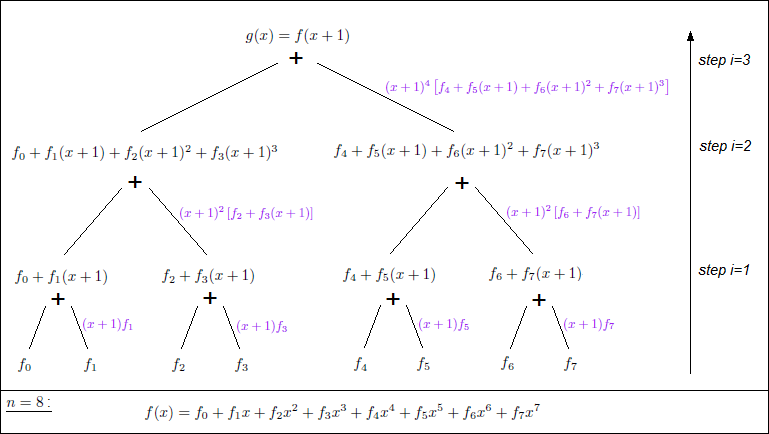
\includegraphics[scale=0.8]{ComputingTree.png}
\end{center}

The first problem we can encounter is the fact it is not simple to make a recursive algorithm in parallel. That's why finally we will consider the tree since its base, i.e. from the coefficients of the input polynomial coefficients. In the C++ code, I did the recursive method, and it was easier to write a method from the base in parallel. In each branch, we see if we need to multiplicate the polynomial evaluated at the base by a monomial shift or not. We see that for each step, the parallelism can be obtained easily. Now the difficulty is to work step by step, consider the good sizes of the arrays, the number of polynomials, the position of the coefficients we're modifying, how to do that the fastest possible.


\subsection{Compute the $(x+1)^{2^i}$}

\subsubsection{Idea}

To compute the serie of $(x+1)^{2^i}$, we have different ways to proceed. But all the classic ways are not necessary the best to compute all the coefficients. \\

If we need all the $(x+1)^j$ for $j \in \mbox{\textlbrackdbl} 1, n\mbox{\textrbrackdbl}$, it will be better to use the formula ${n+1 \choose k+1} = {n \choose k} + {n \choose k+1}$ to compute each element and proceed to a divide and conquer method to compute in parallel the coefficients. But, we just need the coefficients of $(x+1)^{2^i}$. Then, if we proceed with a divide and conquer on all the elements of $(x+1)^j$ and just keep the $(x+1)^{2^i}$, we can have a lot of computations, in particular for $i$ big, which won't be stored and just be needed to go to the next power of $(x+1)$. That's not what we want, so we will use the formula of the binomial coefficients with the factorial sequence to get directly the coefficient of each $(x+1)^{2^i}$. \\

With the method I will explain in this part, I think we loose a little time at the beginning, computing yet the factorial sequence in parallel. But after, the computations are fast and nothing is superfluous.\\

So, to compute the Newton's binomial coefficients, we want to use the following formula :
$$\forall n\in \mathbb{N},\, (x+1)^n = \sum_{k=0}^{n} {n \choose k}\, x^k \mbox{ with } {n \choose k} = \cfrac{n!}{k!\, (n-k)!}$$

We need so to compute all the elements $i! \forall i\in \mbox{\textlbrackdbl} 0, n\mbox{\textrbrackdbl}$.

\subsubsection{The sequence of factorials}

To use the previous formula to get all the binomials' coefficients, we need the values of each $i! \mod p$ for $i \in \mbox{\textlbrackdbl} 0, n\mbox{\textrbrackdbl}$.

One may notice that to obtain $i!$, we need $(i-1)!$. So if we consider the computation in serie of all the $i!$, it may be very long to obtain $n!$ for $n$ big. \\

First of all, we need an array of size $n+1$, called \textit{Factorial\_device} in my code as we also need $0!$. But we don't really need to compute $0! = 1$ so we'll consider the following computations on \textit{Factorial\_device + 1} thus we just compute $i!$ for $i \in \mbox{\textlbrackdbl} 1, n\mbox{\textrbrackdbl}$. Now we consider computations of size $n = 2^e$ with $e \in \mathbb{N}^*$. As $n$ is a power of $2$, I was looking for a code to compute pairwise elements.

\subsubsection{Mapping for the computation of the factorial sequence}

To understand the code, see the following picture from the bottom which is the first step : the initialization. First we initialize the array \textit{Factorial\_device + 1} letting the even elements as their position and we do multiplications on the odd elements. \\

Then, in each step, we consider the array per parts. We can see a part in each step as the following : we multiply the element of a position by a same number for a part, these 'same numbers' are what I call "pillar factors", represented by the darkest boxes. We can see that step after step, we compute several $i!$ in parallel and finally get every $i!$ in $\log_{2}(n)$ steps.\\

\begin{center}
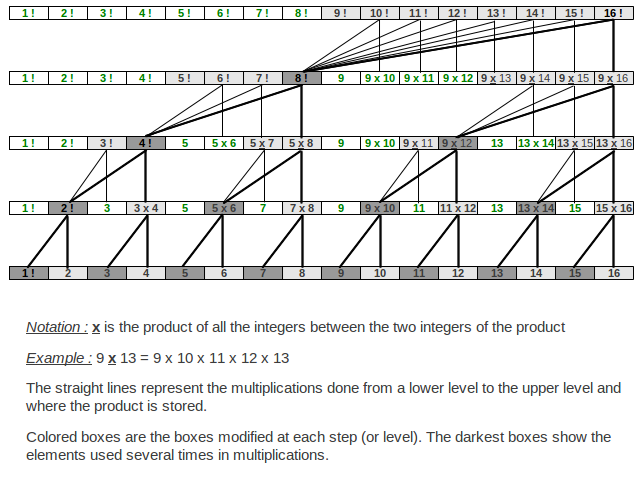
\includegraphics[scale=0.8]{facto.png}
\end{center}

See in the \textbf{Appendix} the file \textit{Taylor\_shift\_kernel.cu} and in particular the procedures \textit{identity\_GPU}, \textit{create\_factorial\_step0\_GPU} and \textit{create\_factorial\_stepi\_GPU} which correspond to the different steps of the computation in parallel of the sequence of factorials. First we inialise the $n+1$ positions in the array \textit{Factorial\_device} with their position or 1 for \textit{Factorial\_device[0]} with \textit{identity\_GPU} and then the two others procedure modified $n/2$ positions of the array at each step. The procedure \textit{create\_factorial\_stepi\_GPU} has only one problem, if we take a look at the previous graphic we can see that in each step, a lot of threads will need the same "pillar factor", so many threads will take the value of a same position in the array at the same time, there is an overlap reducing performances of the code. This part needs to be worked to find another way to do the computation of the factorial elements to improve a little more the efficiency of my code.

\subsubsection{The array of the $(x+1)^{2^i}$}
To do the Taylor shift by 1, we need to compute all the $(x+1)^{2^i}$ as we said before. As now we have the sequence of the factorials, we can compute in parallel each coefficient of the $(x+1)^{2^i}$  but do we we really need all of them ? \\

If we look at the following Pascal triangle until the binomial coefficients of $(x+1)^{8}$, naively we just need to use the coefficients colored in yellow. But, a lot of them are $1$, we can avoid to have too much ones in the array. Moreover, we don't really need $(x+1)^0$. We want also to store these coefficients in an array of $1$ dimension so successively. If we store the coefficients naively, we will store the following sequence : $1,1,1,1,2,1,1,4,6,4,1,1,8,28,56,70,56,28,8,1$. We have to keep in mind also that when we will need to use $(x+1)^{2^i}$, we will need to know the position of this $(x+1)^{2^i}$ in our array. \\

\begin{center}
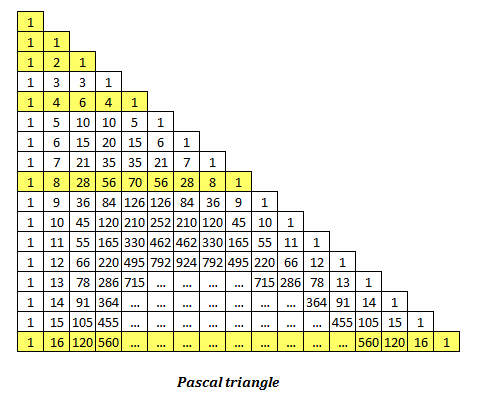
\includegraphics[scale=1]{PascalTriangle.png}
\end{center}

Now, if we avoid all the ones in the first column of the Pascal triangle (except the first for $(x+1)^0$, even though it is useless), the sequence to store becomes : $1,1,2,1,4,6,4,1,8,28,56,70,56,28,8,1$. This sequence is better as the coefficients of $(x+1)^{2^i}$ are easily found at the position $2^i-1$ (except for the first but keep in mind it is useless). Thus, most of the ones in this sequences can be used to represent two consecutives $(x+1)^{2^i}$.\\

Moreover, for a polynomial of degree $n$, this array is of size... $n$ ! So like this, this array will be very practical to use. For $n = 16 = 2^4$, we will use the following array :\\

\begin{center}
\begin{tabular}{|c||c||c|c||c|c|c|c||c|c|c|c|c|c|c|c||} \hline
1 & 1 & 2 & 1 & 4 & 6 & 4 & 1 & 8 & 28 & 56 & 70 & 56 & 28 & 8 & 1 \\ \hline
\end{tabular}
\end{center}

This array is called \textit{Monomial\_shift\_device} in the code and created by the procedure \textit{develop\_x\_shift}. Each thread need first of all to know what $(x+1)^{2^i}$ it deals with and after the coefficient it needs to compute with the function \textit{create\_binomial2\_GPU}.\\

One may notice that if we think more on how to reduce computations, the Pascal triangle is symmetric. So approximatively the half of the coefficients don't really need to be stored as I do for the moment. For example, in the case $n=16$ I have taken, we could just store $1,2,4,6,8,28,56,70$ which will be an array of size $n/2$ and after find a way to use this smaller array correctly to use the coefficient. It is possible and it is a way of reflection I keep in mind when we will try to improve our code when it will be completely finished.\\


\newpage
\section{First steps : for a polynomial of degree $2$ to $512$}
\subsection{The beginning}
First of all, we need to have in input the different coefficients of the polynomial we want to be shifted by $1$. I made a code called \textit{aleaPol.cpp} to create random polynomials of the size wanted. This code stores the coefficients created in a file line per line. So the input is a file we need to read in sequence and then store its data in an array to begin our program. To do that has obviously a cost in time which increases with the size of the polynomial. The way to store efficiently the polynomials is also a question we must ask.\\

At the beginning of the Taylor shift, after the array \textit{Monomial\_shift} was built, we need to copy the array \textit{Polynomial} for the device and then do the first step, which is very simple, this is done by the procedure \textit{init\_polynomial\_shift\_GPU}.\\

Since the second step, computations become less obvious.

\subsection{Next steps, how we proceed}
Let us recall what we have to do. In each step of the previous tree we saw before. In each step, the half of the branches need to be multiplicated by $(x+1)^{2^i}$, $i$ being the current step. Then the result must be added with the previous polynomials of each branch and all of this in parallel in each part of the tree. First of all, we need to determinate which polynomials we have to multiplicate between us. This is what we do with the procedure \textit{transfert\_array\_GPU}. This procedure stores in the array \textit{Mgpu} the polynomials we need to be multiplicated, at a little difference we will explain with the following procedure.\\

\subsection{The plain multiplication \& the right shift}
Now I want to multiplicate in parallel all the polynomials I have stored in \textit{Mgpu}. A member of the laboratory, Anis Sardar Haque has implemented a very efficient multiplication called \textit{listPlainMulGpu} of a list of polynomials I wanted to use for its efficiency. I need to be careful with this because the use I want to do with it is different from the use done by other codes written by the laboratory. So, I face to different problems.\\

Before seeing these problems, let us explain how works exactly \textit{listPlainMulGpu} :\\

\textit{listPlainMulGpu} do pairwise products of polynomials of the same size in a list containing these polynomial. For example, an array may contain the coefficients of eight polynomials called $P_i$ for $i\in \mbox{\textlbrackdbl} 0, 7\mbox{\textrbrackdbl}$ with \textit{listPlainMulGpu}, we can multiply in parallel four products : the products $P_0\times P_1$, $P_2\times P_3$, $P_4\times P_5$ and $P_6\times P_7$. To do that, we need in particular in parameter the array containing the polynomials to multiply (\textit{Mgpu1}), the array which will contain the products (\textit{Mgpu2}), the size of the polynomials \textit{length\_poly}, the number of polynomials called \textit{poly\_on\_layer} (for our example $poly\_on\_layer=8$), the number of threads used for on multiplication, the number of multiplications in a thread block, and obviously $p$ and its inverse for computations modulo $p$. If \textit{Mgpu1} contains $k$ polynomials of size $m$ then \textit{Mgpu1} is of size $k\times m$) and \textit{Mgpu2} contains $k/2$ polynomials of size $2m-1$ so \textit{Mgpu2} is of size $\cfrac{k}{2}\times (2m-1)\neq k\times m$.\\

So, for example after the plain multiplication, the following array \textit{Mgpu1} of size\\
$$poly\_on\_layer \times lenght\_poly = 8 \times 128 = 1024\,:$$

\begin{center}
\begin{tabular}{|c|c||c|c||c|c||c|c|}
\hline
$P_0$ & $P_1$ & $P_2$ & $P_3$ & $P_4$ & $P_5$ & $P_6$ & $P_7$ \\
\hline
\end{tabular}
\end{center}

becomes the following array \textit{Mgpu2} of size\\
$$\cfrac{poly\_on\_layer}{2} \times (2\times lenght\_poly - 1) = 4 \times 255 = 1020\,:$$

\begin{center}
\begin{tabular}{|c|c|c|c|}
\hline
$P_0 \times P_1$ & $P_2 \times P_3$ & $P_4 \times P_5$ & $P_6 \times P_7$ \\
\hline
\end{tabular}\\
\end{center}

Now, let us explain what are the problem we face. \\

First of all, the multiplications we want to do are not between polynomials of the same size. If we look at the tree of computations, we can see that we have to multiply a polynomial $P(X)=\sum_{i=0}^{n-1} a_i\,X^i$ of size $n=2^k$ by $(X+1)^n$, we obtain a polynomial of size $2^{k+1}$ but $P(X)$ and $(X+1)^n$ have for size respectively $n$ and $n+1$. So, to use the multiplication, either we can put zeros on polynomials to have the same sizes (but we will have a lot of multiplications by zeros which will be useless), or we think another way to use the multiplication. \\

Secondly, the initial code of the plain multiplication considered the output array has a modified size as I show that in the previous arrays (size of $1024$ for the first and $1020$ for the second). My objective is to keep the same size as the product of my polynomials are different and allow me to keep at each step polynomial sizes as a power of $2$.\\

So I clearly need to modify this procedure a little to adapt it for what I want to do with. My idea was the following :\\

I decompose the multiplication in another multiplication, a right shift and an addition. As we need the Newton's binomial coefficients, the way to store them I used before was a power of $2$. Consider $local\_n = 2^k$ : $$\forall j\in \mbox{\textlbrackdbl} 0, local\_n - 1\mbox{\textrbrackdbl},\; Monomial\_shift[local\_n + j] = {local\_n \choose j + 1}$$
so at \textit{Monomial\_shift + local\_n}, we store the coefficients of $[(X+1)^{local\_n} - 1]/X$, this polynomial is of size $local\_n$ and thus I want to use this polynomial instead of $(X+1)^m$ for the multiplication. \\

To understand what we can do, imagine we have to multiply locally a polynomial $Q(X)$ of size $m=2^k$ by $(X+1)^{m}$, let us decompose $Q(X) \times (X+1)^{m} 
$ and see how to proceed according to the following to compute $Q(X) \times (X+1)^{m}$ :\\

\begin{align*}
Q(X) \times (X+1)^{m} 
&= \left( \sum_{i=0}^{2^k-1} a_i\,X^i\right) \times (X+1)^{2^k}\\
&= Q(X) \times \left[(X+1)^{m} - 1 + 1 \right]\\
&= Q(X) \times \left[(X+1)^{m} - 1\right] + Q(X)\\
&= Q(X) \times X \times \cfrac{(X+1)^{m} - 1}{X} + Q(X)\\
&= X \times \left( Q(X) \times \cfrac{(X+1)^{m} - 1}{X} \right) + Q(X)
\end{align*}\\

So let us keep in mind the formula obtained :

$$Q(X) \times (X+1)^{m} = X \times \left( Q(X) \times \cfrac{(X+1)^{m} - 1}{X} \right) + Q(X)$$

This formula is very interesting because it allows to solve the problems I explained before. Let us explain why. The polynomials $Q(X)$ and $[(X+1)^{m} - 1]/X$ are of the same size $m$ so can be computed with the plain multiplication described before. Then, as it is not what we really want, we nedd to multiply the result by $X$ which corresponds for our arrays to a right shift of all the coefficients computed, then I won't need to decrease of $1$ the size of each product if I do the right shift within this procedure. And then, we just need to add the previous value of $Q$ to get the result we wish. I called this procedure modified \textit{listPlainMulGpu\_and\_right\_shift}. Just see now a concrete example.\\

\textit{\textbf{Example :}} 
We want to compute $(3+4x) \times (x+1)^2$.\\
Then we store the following coefficients in the array \textit{Mgpu1} : $[3,4,2,1]$.\\
If we write what happens, this is : \\

\begin{align*}
(3+4x) \times (x+1)^2 &= x\,[(3+4x) \times (2+x)] + (3+4x) & \mbox{ decomposition to simplify the problem }\\
&= x\,(6+11x+4x^2+0x^3) + (3+4x) & \mbox{ plain multiplication done }\\
&= (0+6x+11x^2+4x^3) + (3+4x) & \mbox{ right shift done }\\
&= 3+10x+11x^2+4x^3 & \mbox{ addition done }\\
\end{align*}

\textit{listPlainMulGpu\_and\_right\_shift} do the product giving $6+11x+4x^2$ and store it like this $[0,6,11,4]$ so we have done the right shift for the multiplication by $x$ (I write useless zeros in the calculations to show they correspond to a position in the array \textit{Mgpu2}), then we just need to sum with the polynomial, we notice that we just need to sum the half of the coefficients, to do that, I will use the procedure called \textit{semi\_add} I explain in the following part.


\subsection{Partial additions}

As we just saw in the previous part, at the end, we need to add the missing parts $Q(X)$ to obtain exactly the products we want. If we look precisely at these additions, we don't really need to add all the positions of the arrays. Indeed, if we look at the previous example, just the half of the coefficients of the polynomial where added to $Q(X)$ as the size of the $Q(X)$ is the half of the sizes of the polynomials obtained with the procedure \textit{listPlainMulGpu\_and\_right\_shift}. Now we have really multiplied the half of the branches of the current step, we have to add the polynomials computed in these branches with the polynomials of the branches where there were not any multiplication to do.\\

So, to sum up, semi\_add adds the elements $Q(X)$ which were missing to do correctly $Q(X) \times (X+1)^{2^i}$ and then adds in some way $P^{(0)}$ with $P^{(1)}\times (X+1)^{2^i}$ (with $Q = P^{(1)}$). This ends a loop. For the next loop, we do the same with polynomial sizes increased by $2$ and a number of polynomials considered to be multiplicated divided by $2$. This corresponds respectively to $local\_n *= 2$ and $polyOnLayerCurrent /= 2$.\\

\subsection{The arrays}

Some arrays are used in all what I have described before. But let us explained exactly the choice of these arrays and what each array does exactly.\\

At the first step, the array \textit{Polynomial\_device} contains all the coefficients defining the polynomial we want to be shifted. Inside this array, the coefficients are store in the increasing order of the power of $x$.\\
We do then the first step of the tree in the array \textit{Polynomial\_shift\_device[0]} which must contain at the end of the loop the polynomials for the next step.\\

Since the second step, the array \textit{Mgpu} contains exclusively all the polynomials which need to be multiplicated pairwise. For example, at the step 2, let us consider the array :\\

\begin{center}
Polynomial\_shift\_device[0] = \begin{tabular}{|c|c||c|c||c|c||c|c|}
\hline
1 & 2 & 3 & 4 & 5 & 6 & 7 & 8 \\
\hline
\end{tabular}
\end{center}


Then, some polynomials of size 2 inside need to be multiplicated by $(x+1)^2$ so we store in \textit{Mgpu} :\\
\begin{center}
Mgpu = \begin{tabular}{|c|c||c|c||c|c||c|c|}
\hline
3 & 4 & 2 & 1 & 5 & 6 & 2 & 1 \\
\hline
\end{tabular}
\end{center}


We store then the result of \textit{listPlainMulGpu\_and\_right\_shift} in \textit{Polynomial\_shift\_device[1]}. To complete this array, we add the missing part to have exactly $Q(X) \times (X+1)^{2^i}$ so we add parts of \textit{Polynomial\_shift\_device[0]} with \textit{Mgpu}, and then to finish we complete \textit{Polynomial\_shift\_device[1]}, ready for the next step.\\

Before to comment the other step, one can see that at each step since now, we just need the previous\\ \textit{Polynomial\_shift\_device[i-1]} to compute \textit{Polynomial\_shift\_device[i]} (and a new \textit{Mgpu}). We don't need to keep all these arrays, but just the previous one at each step so to avoid useless arrays and costly cudaMalloc, I modified my code to just use \textit{Polynomial\_shift\_device[i\%2]} and \textit{Polynomial\_shift\_device[(i+1)\%2]} so that finally in each step we invert \textit{Polynomial\_shift\_device[0]} and \textit{Polynomial\_shift\_device[1]}. Thus, whatever is the size of the polynomial we consider at the beginning, we have the same number of arrays in the code, at least before the step $10$.\\

Now, we come in a new part of the code. The plain multiplication implemented by the laboratory is very efficient for multiplicate polynomials of degrees at most the number of threads in a thread block, so for polynomials of degrees 512 for my machine. This multiplication can't be done for polynomials of degree size more than 512, at least, it can't be sufficiently efficient. Then we need to proceed differently. For bigger degree, we need to use FFT. The Section 5 explain what it is exactly and how we use it.


\newpage
\section{Fast Fourier Transform (FFT)}
%%%%%%%%%%%%%%%%%%%%%%%%%%%%%%%%%%%%%%%%%%%%%%%%%%%%%%%%%%%%%%%%%
\begin{frame}[fragile]
\frametitle{\textbf{\textcolor{orange}{First definition}}}

\begin{Definition}
Let $n$ be a positive integer and $\omega \in R$.
\begin{itemize}
\item[\textbullet] $\omega$ is a \textcolor{violet}{$n$-th root of unity} if $\omega^{n} = 1$.
\item[\textbullet] $\omega$ is a \textcolor{violet}{primitive $n$-th root of unity} if :
\begin{itemize}
\item[(1)] $\omega^{n} = 1$.
\item[(2)] $\omega$ is a unit in $R$.
\item[(3)] $\forall t$ prime s.t. $t|n$, $\omega^{n/t} - 1$ is neither $0$ nor a $0$ divisor.
\end{itemize}
\end{itemize}
\end{Definition}

We now take $\omega \in R$ to be a primitive $n$-th root of unity.

\end{frame}

%%%%%%%%%%%%%%%%%%%%%%%%%%%%%%%%%%%%%%%%%%%%%%%%%%%%%%%%%%%%%%%%%
\begin{frame}[fragile]
\frametitle{\textbf{\textcolor{orange}{Discrete Fourier transform (DFT)}}}

\begin{Definition}
The $R$-linear map
$$\textcolor{darkgreen}{DFT_{\omega} : \begin{cases}
R^n &\rightarrow R^n \\
f &\mapsto (f(1), f(\omega), f(\omega^{2}),\dots,f(\omega^{n-1}))
\end{cases}}$$
which evaluates a polynomial at the powers of $\omega$ is called the \textcolor{red}{\textbf{Discrete Fourier Transform (DFT)}}.
\end{Definition}

\begin{prop}[consequence of the Lagrange's theorem]
The $R$-linear map $DFT_{\omega}$ is an isomorphism.
\end{prop}

Then we can represent a polynomial $f$ by the \textit{DFT} representation with $\omega$ determined in our code.

\end{frame}
%%%%%%%%%%%%%%%%%%%%%%%%%%%%%%%%%%%%%%%%%%%%%%%%%%%%%%%%%%%%%%%%%

%%%%%%%%%%%%%%%%%%%%%%%%%%%%%%%%%%%%%%%%%%%%%%%%%%%%%%%%%%%%%%%%%
\begin{frame}[fragile]
\frametitle{\textbf{\textcolor{orange}{Convolution}}}

\begin{Definition}
The \textcolor{violet}{\textbf{convolution}} w.r.t. $n$ of $f = \sum_{0\leq i < n} f_i\,x^i$ and $g = \sum_{0\leq i < n} g_i\,x^i$ in $R[x]$ is $h = f*g = \sum_{0\leq k < n}h_k\, x^k$ s.t.
$$\textcolor{darkgreen}{\forall k \in \mbox{\textlbrackdbl} 0, n-1\mbox{\textrbrackdbl},\; h_k = \sum_{i+j\equiv k \mod n}f_i\,g_j}.$$
\end{Definition}

\begin{block}{}
One can prove that $\textcolor{violet}{fg = f*g \mod (x^n-1)}$.
\end{block}

\begin{Lemma}[DFT product amounts to a scalar product]
For $f,g \in R[x]$ univariate polynomials of degree less than $n$ we have 
$$\textcolor{red}{DFT_{\omega}(f * g) = DFT_{\omega}(f)DFT_{\omega}(g)}.$$
\end{Lemma}


\end{frame}
%%%%%%%%%%%%%%%%%%%%%%%%%%%%%%%%%%%%%%%%%%%%%%%%%%%%%%%%%%%%%%%%%

%%%%%%%%%%%%%%%%%%%%%%%%%%%%%%%%%%%%%%%%%%%%%%%%%%%%%%%%%%%%%%%%%
\begin{frame}[fragile]
\frametitle{\textbf{\textcolor{orange}{FFT Maping}}}

\begin{Definition}
The \textcolor{red}{\textbf{Fast Fourier Transform (FFT)}} is an efficient algorithm to compute \textit{DFT} and its inverse. 
\end{Definition}

We use the \textcolor{violet}{Cooley-Tukey} algorithm following a \textit{D{\&}C} strategy.
\begin{center}
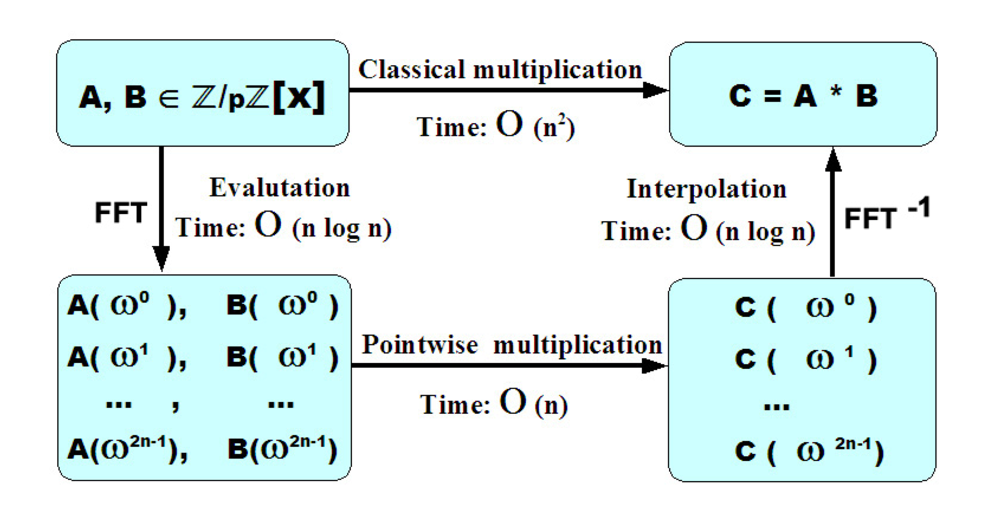
\includegraphics[scale = 0.2]{FFT.png}\\
\small\textbf{FFT-based univariate polynomial multiplication over $\mathbb{Z}/p\mathbb{Z}$}\\
\end{center}

\end{frame}
%%%%%%%%%%%%%%%%%%%%%%%%%%%%%%%%%%%%%%%%%%%%%%%%%%%%%%%%%%%%%%%%%


\newpage
\section{Benchmarks}
First of all, to be sure that the Taylor shift by 1 was done correctly, I needed some comparison, like using Maple, or other codes, in particular in C++. I used mainly the comparison of my CUDA code with the execution of the Horner's method in C++, which is the fastest compared to the Divide and Conquer method in C++ and the execution on Maple. \\

In the following graphics, MAPLE is not represented because the execution time increases by a factor of 4 each time we multiply by 2 the number of coefficients of the polynomial we want to be shifted by 1. Nevertheless, I show the execution time of the Maple script I used in the array of the execution times. \\

Here are the differents results obtained for different sizes of random polynomials. Let us recall that these polynomials are of degree $n = 2^e-1$ : \\

\begin{center}
\begin{tabular}{||c|c||c||r|r||r||}
   \hline
  \multicolumn{6}{||c||}{Execution time in seconds} \\
 \hline
  e  &    n    &    GPU     &  CPU : HOR  &   CPU : DNC  &  Maple 16   \\  \hline \hline
  3  &      8  &  0.001518  &   0.000128  &    0.000141  &     <0.001  \\
  4  &     16  &  0.001432  &   0.000186  &    0.000172  &     <0.001  \\
  5  &     32  &  0.001590  &   0.000167  &    0.000191  &     <0.001  \\
  6  &     64  &  0.001773  &   0.000192  &    0.000294  &      0.008  \\
  7  &    128  &  0.002016  &   0.000261  &    0.000628  &      0.024  \\
  8  &    256  &  0.003036  &   0.000593  &    0.002331  &      0.084  \\
  9  &    512  &  0.002624  &   0.001278  &    0.006304  &      0.320  \\
 10  &   1024  &  0.005756  &   0.005940  &    0.032073  &      1.400  \\
 11  &   2048  &  0.009317  &   0.015312  &    0.095027  &      5.640  \\
 12  &   4096  &  0.013475  &   0.076866  &    0.376543  &     24.478  \\
 13  &   8192  &  0.019674  &   0.324029  &    1.498890  &    104.438  \\
 14  &  16384  &  0.027229  &   1.282708  &    6.861433  &    437.848  \\
 15  &  32768  &  0.042561  &   5.110919  &   23.907799  &   1781.427  \\
 16  &  65536  &  0.064306  &  15.184347  &  114.988129  &   7407.063  \\
 17  & 131072  &  0.127214  &  80.625801  &  477.934692  &     >10000  \\
   \hline 
\end{tabular}
\end{center}

To compare more in details, take a look at the differents pictures we can have using gnuplot. Gnuplot scripts can be seen in the appendix. The execution times of MAPLE 16 don't appear as they increase too much compared to my other results. I show different graphics, considering $e$ in x-axis then $n$, as my results are for polynomials of size $2^e$. The results with $n$ in x-axis are more eloquent concerning the fact that the execution time becomes linears when $n$ increases by a factor of $2$.\\

\begin{center}
\textbf{Execution time of the GPU in function of $e$}
\end{center}

\begin{center}
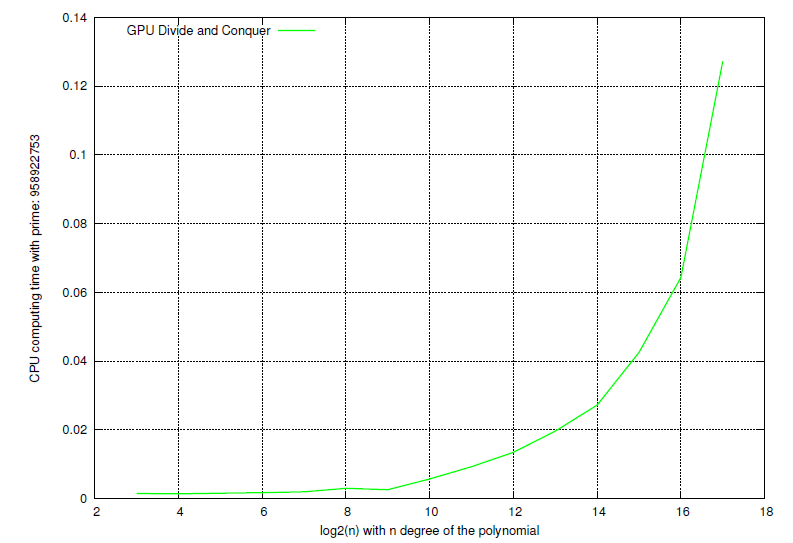
\includegraphics[scale=0.8]{eps/GPUtime_e.png}
\end{center}

The following graphic is more eloquent concerning the linear increasing of the execution time of the GPU depending on the power of $2$ the size of the polynomial is considered :\\

\begin{center}
\textbf{Execution time of the GPU in function of $n$}\\
\end{center}

\begin{center}
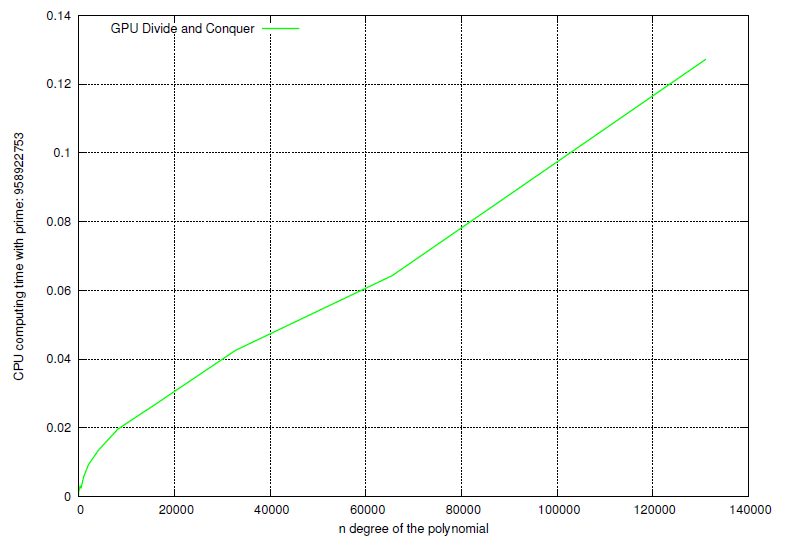
\includegraphics[scale=0.8]{eps/GPUtime_n.png}
\end{center}

Now let's take a look at the execution times for the Horner's method and for the Divide and Conquer method in serie, so with the CPU only. The two methods increase linearly by scales.\\

\begin{center}
\textbf{Execution time of the CPU in function of $n$}\\
\end{center}

\begin{center}
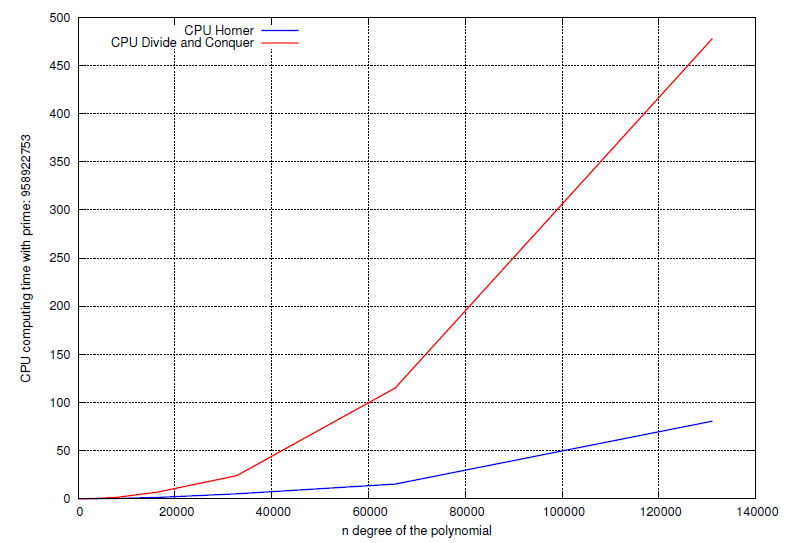
\includegraphics[scale=0.8]{eps/CPUtime_n.png}
\end{center}

We clearly see that the Horner's method in serie is more efficient than the Divide and Conquer method in serie. To see exactly what happen for small degrees and big degree for the three methods, namely the GPU DNC method, the CPU DNC method and the CPU Horner's method (when I say GPU I mean 'in parallel', and when I say CPU I mean 'in serie'). Let's consider the two following graphics.\\


\begin{center}
\textbf{Execution times in function of $n$ for small degrees}\\
\end{center}

\begin{center}
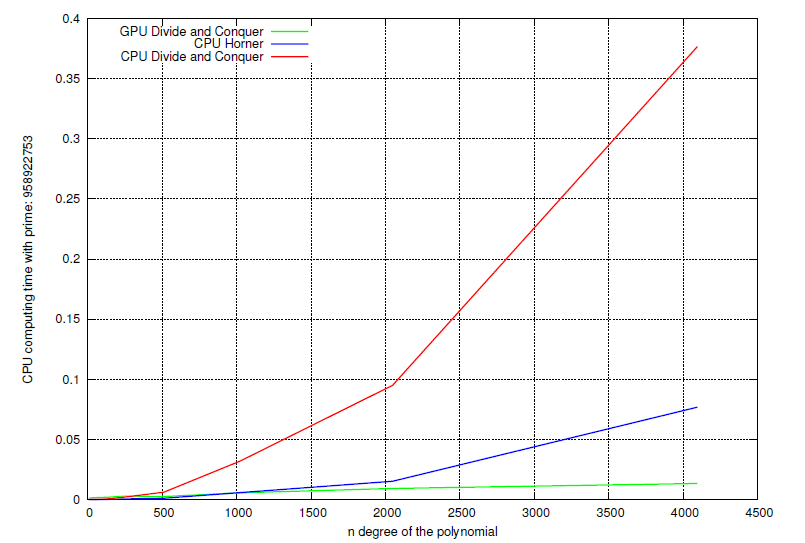
\includegraphics[scale=0.8]{eps/time_small_n.png}
\end{center}

For small degrees, we see that the execution time of the GPU code is approximatively the same and worst than the execution times of the CPU execution times. The reasons are very simple, for small degrees, we need the same number of arrays in the CUDA code than for the big degrees, even though obviously they are not at the same size than for big degrees. Allocate memory for the GPU takes a lot of time at the scale of the execution times for small degrees, so finally there are a lot of communications just for 'small' computations. To conclude with this, for small degrees, it will be better to do the Taylor shift by 1 in serie. There is also the fact that we don't compute the same way the Taylor shift in the three methods, even though for the divide and conquer in serie, the only difference is the way we do the multiplication (and obviously the fact it is in serie).\\

Let's see the comparison for the next degrees :\\

\begin{center}
\textbf{Execution times in function of $n$ for big degrees}\\
\end{center}

\begin{center}
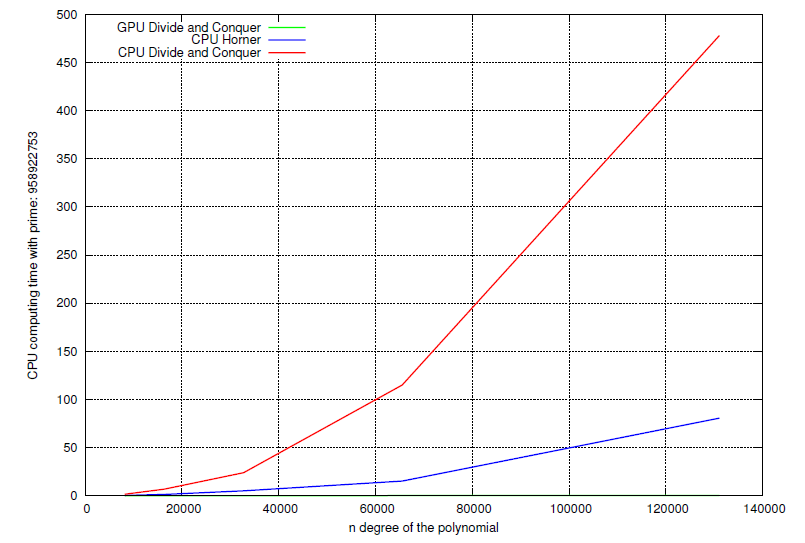
\includegraphics[scale=0.8]{eps/time_big_n.png}
\end{center}

For big degrees, using the GPU gives best performances with a execution time of approximatively 0.1 second for a polynomial of size $2^{17}$.


\newpage
\section*{Appendix}
\subsection{Divide and Conquer Cuda code}
\subsubsection{taylor\_shift.cu}
\lstinputlisting{code/TaylorShift.c}

\subsubsection{taylor\_shift\_cpu.cu}
\lstinputlisting{code/TaylorShiftCpu.c}

\subsubsection{taylor\_shift\_kernel.cu}
\lstinputlisting{code/TaylorShiftKernel.c}

\subsubsection{taylor\_shift\_fft.cu}
\lstinputlisting{code/TaylorShiftFft.c}

\subsubsection{taylor\_shift\_conf.h}
\lstinputlisting{code/TaylorShiftConf.c}

\subsubsection{File calling these procedures : testGPU.cu}
This code calls the procedure taylor\_shift included in the file \textit{taylor\_shift.cu} :
\lstinputlisting{code/testGPU.c}

\subsection{Horner's method C++ code}
\lstinputlisting{code/testHOR.c}

\subsection{Divide and Conquer C++ code}
\lstinputlisting{code/testDNC.c}

\subsection{Maple code}
The procedure we describe in this part makes the taylor shift by one of a polynomial $pp$ of variable $x$ in input modulo $prime$ which is a prime number. We can create a random polynomial $pp$ with the maple instruction \textit{randpoly}, for example :\\
\textit{pp := randpoly($x$, degree = $2^{10} - 1$, terms = $2^{10}$):}\\

Then we can run the following procedure with $pp$ and a prime number we choose ($958922753$ as for the other examples). Here is the procedure : \\

\lstinputlisting{code/xplus1.input}



\newpage
\nocite{*}
\bibliographystyle{plain}
\bibliography{references}


\end{document}
